%!TEX root = ../Manual.tex
\chapter{前言}
\label{Chap_Intro}
本文档是《四川大学学位论文~\LaTeX~模版》的说明文档。


四川大学学位论文的工作以前由~dahakawang\footnote{\url{https://github.com/dahakawang/scu_thesis_template}}~、~tan\footnote{\url{http://www.codeforge.com/article/382397}}~等人做过。本模版是在参考~Casper Ti. Vector\footnote{\url{CasperVector@gmail.com}}~~\emph{pkuthss}~模版\cite{pkuthss}的基础上完成的。


Legendary L.\footnote{Legendary Leo \url{https://github.com/cuiao}}是本文档的创建者和维护者。

\section{特点}
\label{Sect_KeyFeatures}
本模版是严格按照《四川大学硕士、博士学位论文格式》\cite{SCUDissertationFormat}中的要求编写的,有以下几个特点:
\begin{itemize}
	\item 使用简单:本模版在编写之初就考虑到~\LaTeX~初学者的情况,按照本手册的说明,不需要高深的~\LaTeX~知识便可使用本模版进行论文写作。
	\item 自动化程度高:本模版的页码、标题、题注、目录等均使用了自动化命令,一般不需要用户干预。
	\item 写作方便:本模版的主要命令在样式文件中进行了封装,并采用了多文件编译方式。方便用户的写作与修改。
\end{itemize}

\section{推荐配置}
\label{Sect_RecommandedConfiguration}
本模版的使用和正确编译依赖以下几项:
\begin{description}[style=nextline,labelindent=2em,labelwidth=!]
	\item[中文字体] 本模版需要中文字体的支持。
	\item[\TeX~发行版] 一个支持中文的~\TeX~发行版,推荐使用~\TeX~Live\footnote{\url{https://www.tug.org/texlive/}}~,本模版即是使用~\TeX~Live~构建的。
	\item[文本编辑器] 一个好用的文本编辑器有利于你的写作,推荐使用~Atom\footnote{\url{https://atom.io/}}~,必备插件为~atom-latex\footnote{\url{https://github.com/thomasjo/atom-latex}}~和~language-latex\footnote{\url{https://github.com/area/language-latex}}~。
	\item[PDF~阅读器] 一个轻量级的~PDF~阅读器有利于提升效率,推荐使用~SumatraPDF\footnote{\url{http://www.sumatrapdfreader.org/free-pdf-reader.html}}~与~atom-latex~插件联用。
\end{description}


\section{模版文件}
\label{Sect_Files}
本模版根目录\verb|./|下文件夹或文件如下:
\dirtree{%
	.1 ../.
	.2 README.md\DTcomment{自述文件}.
	.2 Template\DTcomment{模版文件夹}.
	.2 MainBody\DTcomment{论文主体文件夹}.
	.2 Manual\DTcomment{手册(本文档)文件夹}.
}
其中,\verb|Template|(模版文件夹)较为重要,一般情况下请勿修改!以下按上述文件夹分类介绍本模版中的文件。

\subsection{模版文件夹}
\label{Subsect_TemplateFolder}
\verb|Template|为本模版最重要的文件夹,用于存放本模版的样式、宏定义、资源等文件,一般情况下请勿修改!详细的文件目录如下:
\dirtree{%
	.1 Template.
	.2 scuthesis.cls\DTcomment{模版样式文件}.
	.2 scuthesis.def\DTcomment{模版宏定义文件}.
	.2 chinesebst.bst\DTcomment{中文参考文献样式文件}.
	.2 Components.
	.3 Images.
	.4 SCU{\_}TITLE.eps\DTcomment{四川大学~LOGO}.
}

\subsection{论文主体文件夹}
\label{Subsect_MainbodyFolder}
\verb|MainBody|~文件夹主要用于填写论文内容,用户可以方便地将自己的论文按照章节填写到此文件夹中。详细的文件目录如下:
\dirtree{%
	.1 MainBody.
	.2 MainBody.tex\DTcomment{主\TeX文件}.
	.2 ReferenceBase.bib\DTcomment{参考文献库文件}.
	.2 Chapters\DTcomment{章节文件夹}.
	.3 0{\_}0{\_}Abstract.tex\DTcomment{中英文摘要}.
	.3 0{\_}1{\_}Abbreviations.tex\DTcomment{缩略词表}.
	.3 0{\_}2{\_}Symbols.tex\DTcomment{符号表}.
	.3 Introduction.tex\DTcomment{引言}.
	.3 Chapter2.tex\DTcomment{第二章}.
	.3 Thanks.tex\DTcomment{致谢}.
	.3 Achievements.tex\DTcomment{科研成果}.
	.3 CopyrightAuthorization.tex\DTcomment{版权授权(请勿修改)}.
	.3 OriginalStatement.tex\DTcomment{原创声明(请勿修改)}.
}
以上文件除~\verb|CopyrightAuthorization.tex|~和~\verb|OriginalStatement.tex|~按照学校统一的内容和格式规定禁止修改外,其他均可按照用户的需要进行修改。\\
\verb|ReferenceBase.bib|~可使用~\emph{EndNote\textsuperscript{\texttrademark}}~这类文献管理工具导出。


若~\verb|Chapters|~文件夹有改动,请使用~\verb|\include{Chapters/<文件名>}|~命令在~\verb|MainBody.tex|~做相应的修改(即若在~\verb|Chapters|~中增加了文件~\verb|Chapter3.tex|~,对应在~\verb|MainBody.tex|~的命令为~\verb|%!TEX root = ../MainBody.tex

%第三章
\chapter{需求分析}
共享经济的发展如火如荼 \cite{SharingEconomy2},图书平均保有量也在稳中增长,在共享图书系统开发之前,需要具体分析用户需求,确保
符合并满足用户的需求。

\section{可行性分析}
在项目开发和需求分析之前,需要系统地分析项目开发和未来交付运行地可行性。

\begin{itemize}
	\item 市场可行性
	
	据统计分析\cite{BookMarketReport2018},2018 年中国全国图书零售市场规模维持两位数增长,2018 年
	中国图书零售市场码洋规模达894亿,同比上升 11.3\%,增速相比 2017 年有所放缓,但依然维持两位数
	增长。新书品种维持平稳,新书定价持续上升。2018 年新书平均单册码洋 41.5 元。
	
	中国图书这么庞大并且持续增长的销售规模,表明人们对于纸质书籍依然有很大的需求,而且表明
	个人手头都有一些已经购买阅读过的闲置书籍。随着纸价的上涨,图书的平均单价也在上涨,这
	也给个人获取书籍增加了不少的成本。如果能够让这些图书在消费者之间流通起来,将大大减少人们的阅读
	成本,从而使人们在相同的成本下能够阅读到更多的书籍,也提高了书籍的利用率,减少了对纸的需求,
	间接保护了生态环境。
	
	本平台将提供消费者之间图书流通的平台,让书籍在人们之间流通起来,看起来是完全可行的。

	\item 技术可行性
	
	目前,以spring开发框架进行后端开发非常流行,而且技术比较成熟,Spring 框架也使得开发 Restful
	形式的服务非常方便。Spring 还集成了 Spring JPA,Spring Security 等子模块,这大大简便了后端
	的开发。Spring 基于 POJO 的开发方式相对与企业级的 Java Bean 也非常轻量级。开发者能够快速掌握 Spring
	后端开发。笔者学习过相关技术,并且曾经使用相关技术做过一个个人博客系统。对相关技术比较了解,所以后端
	开发技术上是可行的。

	前后端分离\cite{backendDispart}的开发方式,思想也比较成熟,并且得到了广泛的应用。前后端的解耦大大加快了项目的开发效率。
	前后端可以约定交互的接口,然后同时进行开发。而且 Spring 只需要简单配置就能够开发 Restful 服务,暴露
	Restful 接口。

	Android 从最初的 Android 1.0,到当前的 Android 9.0 ,API 也非常成熟,资料文档非常齐全。Android 也有
	很多网络库和 Json 库,使得 Android 能够非常容易地访问Restful形式地服务。笔者在寒假之前就开始学习 Android 开发,
	边学习边开发,之前也尝试开发过一些 Demo,所以 Android 端技术上也是可行的。

	所以从技术地角度来讲,是完全可行的一个项目,技术非常成熟,能够迅速进行开发。
	
\end{itemize}



\section{需求概述}
主要的需求是用户的发布图书,并且浏览平台上的闲置图书,并在平台上进行个人
已发布图书基本管理,对他人图书的借阅,归还等。还包括了基础的登录注册功能。总体划分为以下几个功能
模块:

\begin{enumerate}
	\item 首页图书列表,底部包含一个导航,上面显示的是本地缓存的图书列表信息,通过上划,获取更多的图书信息。
	\item 发布图书,点击发布按钮扫描图书条形码或者手动输入图书 ISBN,最终都将图书 ISBN 作为参数,请求服务器,获取服务器返回的图书信息,
	然后用户补充图书信息,例如个人描述,出售租赁价格等,并发布图书。
	\item 最近联系人列表,显示当前用户的最近联系人列表。
	\item 我的首页,显示与我相关的信息选项,包括我的发布,我的钱包,退出登录,清除缓存等。
	\item 我的发布,显示我已经发布的图书列表。
	\item 图书详情,显示图书的详细信息,包括标题,作者,ISBN,描述,出版时间,价格等详细信息。
	\item 我的钱包,显示我的钱包余额。
	\item 注册登录,这是两个不同的界面,一个用来通过邮箱和用户名进行注册,一个用用户名或者邮箱来登录。
	\item 下订单,用户点击图书详情的购买或租赁,进行下单,并转到支付界面。
	\item 支付,用户进行支付。
\end{enumerate}

\section{用户角色}
在该系统中,用户拥有多种角色,包括用户,租书消费者,购书的消费者,书籍拥有者,交付员。当用户注册登录后,便成了该平台的用户。
当用户发布了一本图书,该用户就是一个书籍拥有者,如\cref{owner}。当该书被租出或卖出时,该用户在交付过程中可能成为交付员,如\cref{deliver},负责将图书交付给消费者。
当用户在平台上购买了某本书时该用户是购书消费者,如\cref{costumer}。当用户租了某本书时,用户是租书消费者,如\cref{costumer}。

\begin{figure}[h]
	\centering
	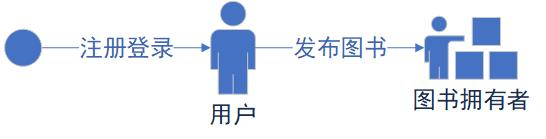
\includegraphics[scale=0.65]{Chapters/UML/owner.jpg}
	\caption{拥有者}
	\label{owner}
\end{figure}

\begin{figure}[h]
	\centering
	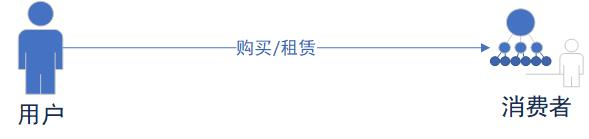
\includegraphics[scale=0.65]{Chapters/UML/costumer.jpg}
	\caption{消费者}
	\label{costumer}
\end{figure}

\begin{figure}[h]
	\centering
	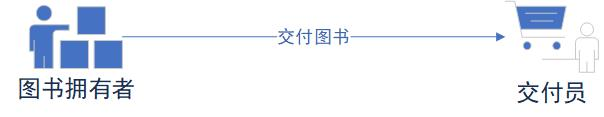
\includegraphics[scale=0.65]{Chapters/UML/deliver.jpg}
	\caption{交付员}
	\label{deliver}
\end{figure}

\section{系统业务流程}
基于 Android 的图书共享系统,需要满足用户基本的登录注册,发布图书,借阅租赁图书,沟通交流的需求。通过手机简单
的扫描图书条形码即可简单的发布图书,在手机上即可浏览图书相关信息,并且通过手机下单进行租赁,购买沟通等
功能。\cref{system_bussness_process}是完整的系统业务流程图。

\begin{enumerate}
	\item 发布图书,用户通过手机客户端扫描或手动输入图书 ISBN,获取到图书信息,进一步补充图书信息,租赁价格,出售价格,
	个人描述,点击发布。
	\item 租赁图书,用户在某本书下通过与主人沟通协商交易信息,就价格和交付方式达成一致后点击租赁,生成订单,进行支付,等待
	交付。租赁期限内,归还图书。订单完成。
	\item 购买图书,在双方协商一致后,下单,支付,交付。订单完成。
	\item 沟通交流,当用于对某本书有兴趣时,可以跟该书主人沟通交流。
\end{enumerate}

\begin{figure}[h]
	\centering
	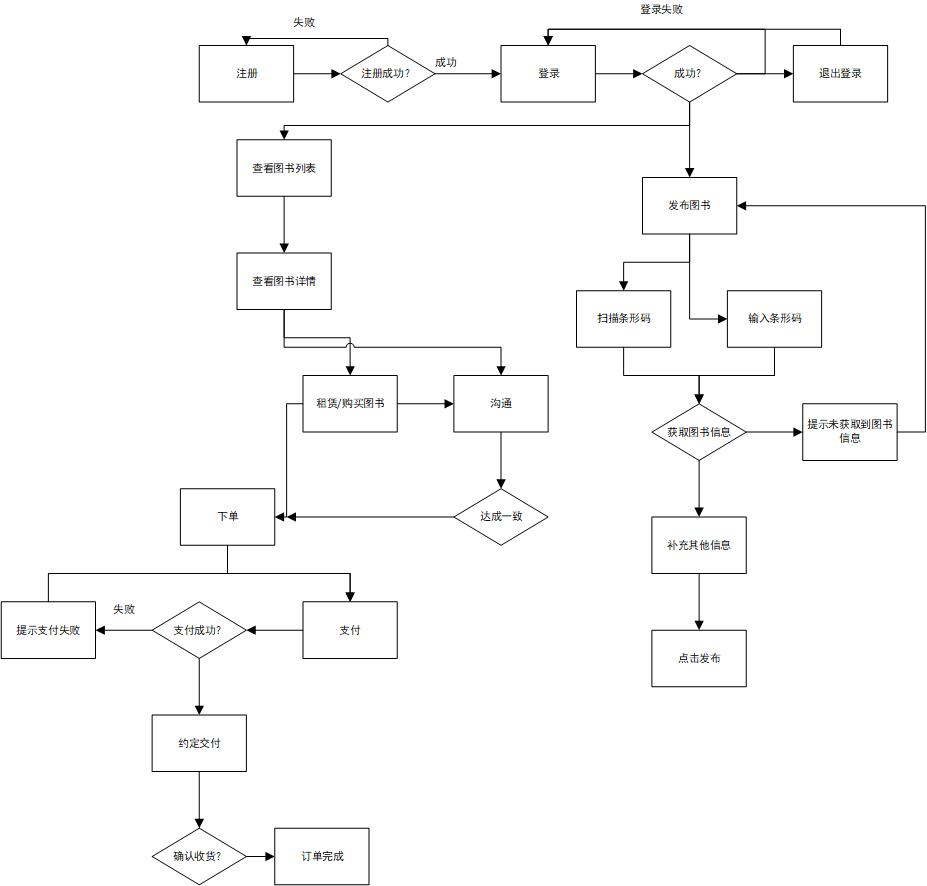
\includegraphics[scale=0.6]{Chapters/UML/system_bussness_process.jpg}
	\caption{系统业务流程图}
	\label{system_bussness_process}
\end{figure}

\section{功能需求}
\cref{function_structure}是功能结构图

\begin{figure}[h]
	\centering
	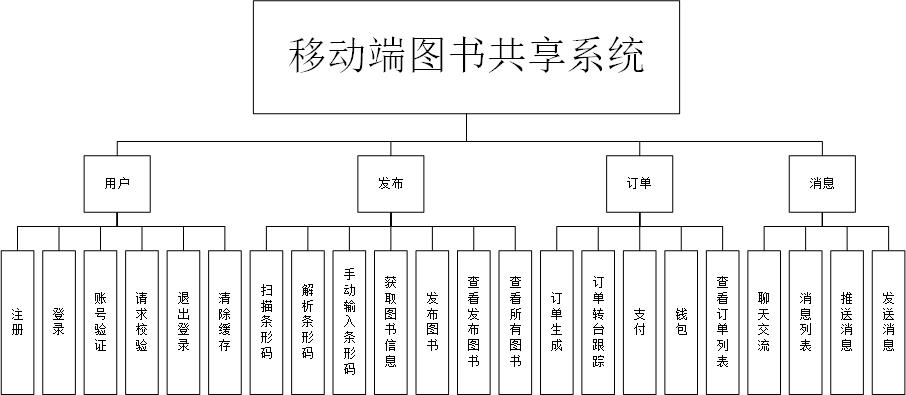
\includegraphics[scale=0.65]{Chapters/UML/function_structure.jpg}
	\caption{功能结构图}
	\label{function_structure}
\end{figure}

\begin{itemize}
	\item 注册, 客户端的用户注册。
	\item 账号验证,用户注册时验证账号是否合法。
	\item 登录,客户端用户登录。
	\item 请求校验,对用户请求的合法性进行角色权限判断。
	\item 扫描条形码,移动端调用详细扫描条形码。
	\item 解析条形码,对扫描到的条形码进行解析。
	\item 手动输入条形码,用户自行输入条形码。
	\item 获取图书信息,根据 ISBN 获取图书相关信息。
	\item 发布图书,客户端完成用户图书的发布。
	\item 订单生成,用户下单,服务器生成相应订单。
	\item 聊天交流,用户之间的沟通协商。
	\item 订单状态跟踪,对订单状态的改变。用户下订单时,订单处于未支付状态。用户支付,订单变为已支付状态。订单交付,订单变为完成状态。
	\item 支付,对订单进行支付,检查用户账户余额,并完成扣款。
	\item 钱包,对用户账户的余额进行操作,增加,扣除。
	\item 查看订单列表,获取用户完整的订单列表。
	\item 查看发布图书,获取用户的所有已发布的图书。
	\item 查看所有图书,获取所有用户发布的所有图书。
	\item 退出登录,完成用户退出操作。
	\item 清除缓存,清除客户端缓存数据。
	\item 消息列表,获取用户的聊天记录。
	\item 推送消息,用户收到来自其他人的消息时,推送消息。
	\item 发送消息,发送给其他用户消息。
\end{itemize}

\section{数据需求}

\begin{itemize}
	\item 用户账户信息,在注册和登录时,用户在客户端完成信息补充。
	\item 图书 ISBN, 通过条形码扫描解析或者用户手动输入获取 ISBN。
	\item 图书详情的 Json 数据,通过客户端获取到的 ISBN,从服务器获取 Json 数据,服务器从 books.googleapis.com 获取关于图书的 Json 数据信息。
	\item 订单数据,用户下单后,服务端应返回完整的订单信息。
	\item 订单列表,从服务器获取单个用户的所有订单信息。
	\item 聊天数据,用户登录后,从服务器获取历史信息。
	\item 钱包数据,查看用户余额。
	\item 用户图书列表,从服务器获取单个用户已发布的图书列表。
	\item 图书列表,从服务器获取所有已发布的图书列表。
\end{itemize}

\section{本章小结}
本章主要完成了共享图书的需求分析,首先对系统开发的可行性进行了分析,从经济可行性、技术可行性两个方面进行
了分析。然后对共享图书的功能需求进行了分析说明。

|~)。更多的使用方法请详见第\ref{Chap_UsingOfThisTemplate}章。

\subsection{手册文件夹}
\label{Subsect_ManualFolder}
\verb|Manual|~是本手册的文件夹,其内容与~\verb|MainBody|~较为类似,在此不做赘述。详细的文件目录如下:
\dirtree{%
	.1 Manual.
	.2 Manual.tex\DTcomment{本手册主\TeX文件}.
	.2 Manualbib.bib\DTcomment{本手册参考文献库文件}.
	.2 Manual.pdf\DTcomment{本手册}.
	.2 Chapters\DTcomment{本手册章节文件夹}.
	.3 0{\_}0{\_}Abstract.tex\DTcomment{中英文摘要}.
	.3 0{\_}1{\_}Abbreviations.tex\DTcomment{缩略词表}.
	.3 0{\_}2{\_}Symbols.tex\DTcomment{符号表}.
	.3 1{\_}Introduction.tex\DTcomment{前言(本章)}.
	.3 2{\_}Using.tex\DTcomment{模版的使用}.
	.3 3{\_}Realization.tex\DTcomment{部分功能实现}.
	.3 Thanks.tex\DTcomment{致谢}.
	.3 Achievements.tex\DTcomment{科研成果}.
	.3 CopyrightAuthorization.tex\DTcomment{版权授权(请勿修改)}.
	.3 OriginalStatement.tex\DTcomment{原创声明(请勿修改)}.
	.3 CopyrightStatement.tex\DTcomment{版权声明(请勿修改)}.
}
